\nonstopmode
% Preamble
  %% Note: you can also specify any of the following options:
  %%  logo: put a University of Edinburgh logo onto the title page
  %%  frontabs: put the abstract onto the title page
  %%  deptreport: produce a title page that fits into a Computer Science
  %%      departmental cover [not sure if this actually works]
  %%  singlespacing, fullspacing, doublespacing: choose line spacing
  %%  oneside, twoside: specify a one-sided or two-sided thesis
  %%  10pt, 11pt, 12pt: choose a font size
  %%  centrechapter, leftchapter, rightchapter: alignment of chapter headings
  %%  sansheadings, normalheadings: headings and captions in sans-serif
  %%      (default) or in the same font as the rest of the thesis
  %%  [no]listsintoc: put list of figures/tables in table of contents (default:
  %%      not)
  %%  romanprepages, plainprepages: number the preliminary pages with Roman
  %%      numerals (default) or consecutively with the rest of the thesis
  %%  parskip: don't indent paragraphs, put a blank line between instead
  %%  abbrevs: define a list of useful abbreviations (see documentation)
  %%  draft: produce a single-spaced, double-sided thesis with narrow margins
  %%

  %% For a PhD thesis -- you must also specify a research institute:
  % \documentclass[phd,ilcc,twoside]{infthesis}
  %% Taught MSc -- specify a particular degree instead. If none is specified,
  %% "MSc in Informatics" is used.
  \documentclass[msc, logo, parskip, abbrevs, notimes, twoside]{infthesis}  % (optional) twoside, draft, leftchapter, doublespacing

  %% Packages used
  \usepackage[svgnames]{xcolor}
  \usepackage[xetex, colorlinks, linkcolor=MediumBlue, citecolor=DarkGreen, urlcolor=MediumBlue, hypertexnames=false]{hyperref}
  \usepackage[hypcap]{caption} % correctly hyperlink captions
  \usepackage{subcaption}
  \usepackage{fontspec}
  \usepackage{subcaption}
  \usepackage{multirow}
  \usepackage{adjustbox}
  \usepackage{booktabs}
  \usepackage{float}
  \usepackage{pdfpages}
  \usepackage{fancybox}
  \usepackage{minted}
  \usepackage{amsmath}
  \usepackage{multirow}
  \usepackage{wasysym}
  \usepackage[titletoc, header]{appendix}
  \usepackage{array}
  \newcolumntype{P}[1]{>{\centering\arraybackslash}p{#1}}
  \setmainfont[Mapping=TeX-text,Ligatures=TeX]{CMU Serif}
  \setsansfont[Mapping=TeX-text,Ligatures=TeX]{CMU Sans Serif}
  % \setmainfont[Mapping=TeX-text,Ligatures=TeX]{Linux Libertine O}
  % \setsansfont[Mapping=TeX-text,Ligatures=TeX]{Linux Biolinum O}
  % \setmainfont[Mapping=TeX-text,Ligatures=TeX]{Baskerville}

  \newcommand{\repeatcaption}[2]{%
    \renewcommand{\thefigure}{\ref{#1}}%
    \captionsetup{list=no}%
    \caption{#2 (repeated from page \pageref{#1})}%
  }

  \newenvironment{shortitemize}
  { \begin{itemize}
    \setlength{\itemsep}{2pt}
    \setlength{\parskip}{3pt}
    \setlength{\parsep}{0pt}
  }
  { \end{itemize}  }

%% Information about the title, etc.
\title{Design \& Implementation of a Password Strength Meter for Partial Passwords}
\author{Vasileios Gerakaris}

%% Optionally, specify the graduation month and year:
% \graduationdate{August 2016}

%% Abstract.
\abstract{
  \emph{Partial passwords} are queries of a subset of character positions from a full password; this authentication scheme is prevalent amongst financial institutions in the UK and is used in both online and telephone banking. Despite being a critical part of financial security, there is insufficient academic research about this mechanism and no known attempts to define accurate metrics for measuring partial password strength.

  In this dissertation, we take a practical approach towards the partial password strength metric. We examine the best available online attack against partial passwords, the \emph{projection dictionary} attack devised by D. Aspinall and M. Just, and use it to define a partial password's strength as the inverse of the likelihood an adversary can successfully guess a partial challenge.

  To the best of our knowledge, no implementation of a password strength meter for partial password exists. We therefore discuss the design choices made and the implementation process followed in creating the first of its kind. In order to evaluate its effectiveness in guiding users towards selecting stronger and more memorable passwords, we conducted an online study. Judging from the obtained results, the display of the developed partial password strength meter is proven to be effective in increasing the security of the chosen partial passwords.
}

\begin{document}
%% Preliminary pages
\begin{preliminary}

  %% This creates the title page
  \maketitle

  %% Acknowledgements
  \begin{acknowledgements}
  Acknowledgements go here.
  \end{acknowledgements}

  %% Next we need to have the declaration.
  \standarddeclaration

  %% Finally, a dedication (this is optional -- uncomment the following line if
  %% you want one).
  % \dedication{To my mummy.}

  %% Create the table of contents
  \tableofcontents

  %% List of figures or tables (optional)
  % \listoffigures
  % \listoftables
\end{preliminary}

% !TEX root = ../msc_thesis.tex

\chapter{Introduction}
  \label{cha:intro}
  This dissertation presents a password strength meter that evaluates passwords' strength against online attacks on partial challenges. We discuss the design choices made behind the implementation and explore its effects on the strength of the selected passwords as well as their memorability.

  \section{Motivation}
    \label{sec:motivation}
    The ubiquity of passwords, as the primary method for user authentication on the internet is undeniable, despite harsh criticism regarding their usability and security~\cite{replace_pass}. For applications where security is of paramount importance (such as banking services), multiple methods of authentication are commonly used.

    \emph{Partial Password} challenges, where users are asked to enter a subset of characters from their selected \emph{memorable information} is such a secondary authentication scheme, commonly used by financial institutions in the UK and, to a lesser degree, in Europe~\cite{2fa_uk}. The topics of cracking user passwords and using password-methods have been thoroughly researched in the past~\cite{pass_strength_empirical,pass_strength}, but the research was focused on traditional passwords.

    Despite their use in security-critical applications, there is little literature concerning attacks on partial passwords and metrics to evaluate their strength. To our knowledge, there does not exist any implementation of a password strength meter for partial passwords; the attempt to design and build the first of its kind is presented within this dissertation.


  \section{Thesis contribution}
    \label{sec:contribution}
    The main contributions of this work are the following:
    \begin{enumerate}
      \setlength{\itemsep}{2pt}
      \setlength{\parskip}{0pt}
      \setlength{\parsep}{0pt}
      \item Survey of the extent of partial passwords' use as an authentication method.
      \item Design \& implementation of a novel strength meter for partial passwords.
      \item Evaluation of the partial password strength meter's effect on the strength and memorability of the selected passwords.
    \end{enumerate}


  \section{Chapter outline}
    \label{sec:outline}
    In Chapter~\ref{cha:background}, we present the theoretical background which is considered important for a reader of this work, in order to comprehend the concepts and designs discussed later. Specifically, we present basic concepts about passwords, partial passwords and attacks against them, briefly explain the ideas behind traditional password strength meters and summarise the results of personal research on how extensively strength meters and partial passwords are used in authentication systems.

    In Chapter~\ref{cha:design_implementation}, we discuss the attacks on partial passwords in more depth, which guide the reasoning behind the design choices made for the partial password strength metrics and the visual presentation of the strength meter. In the second part of the chapter, we present details of the implementation, as well as the website created to showcase and test it.

    In Chapter~\ref{cha:results}, we describe the methodology used to evaluate the effect of the partial password strength meter in the strength of the selected passwords as well as their memorability. We discuss the results of the surveys and draw conclusions regarding our implementation.

    In Chapter~\ref{cha:conclusion}, we mention the known limitations of this work, planned improvements to the implementation, and list some research questions that were raised during the course of the dissertation, some of which the scientific community may deem interesting and wish to explore further.

% !TEX root = ../msc_thesis.tex

\chapter{Background}
\label{cha:background}

  \section{Passwords}
    \label{sec:passwords}
    Passwords are secret strings of characters which have been used as the primary method for both online and offline user authentication in the computing era. They appear in various forms and they are generally classified depending on their allowed character set and length. The term \emph{password} commonly refers to strings of small to average length (6-16 characters), while a \emph{passphrase} is usually a longer string (>20 characters), often a sequence of words. Alphanumeric characters are allowed in passwords and passphrases, and in many cases other ASCII printable characters are included in the available character sets. Passwords created for services often must abide by a \emph{password policy}, a set of requirements enforced by that individual service/organisation, in an effort to increase password strength and security~\cite{pass_policy,NIST_invalid}, as previous research has shown that in the absence of a password policy, users tend to select generally weaker and guessable passwords~\cite{reused_passwords,pass_policy_users_bad}.

    Ideally, passwords must comply with two conflicting requirements: they should be easy to remember and use without writing them down, while at the same time be unique for each service, look random and be hard to guess. This conflict is called the \emph{password problem} and is almost impossible for most users, experts and non-experts alike, who often reuse passwords or write them down to cope with it~\cite{the_password_problem,pass_management}. Komanduri et al. suggested the use of a password policy that is neither too stringent, but at the same time offers noticeable improvements in password strength.

    \subsection{Partial passwords}
      \label{ssec:partial_passwords}
      \emph{Partial password} was defined by D. Aspinall and M. Just~\cite{part_pass}:
      \begin{quote}
      A \emph{partial password} is a query of a subset of characters from a full password, posed as a challenge such as ``Give me letters 2, 3 and 6 from your password''.
      \end{quote}
      Throughout this dissertation we use a slightly different terminology; the term \emph{partial password challenge} is used to refer to such queries, and we use the term \emph{partial password} to refer to passwords on which \emph{partial password challenges} will be issued. The idea behind partial password challenges is that an adversary that observes a user answering the challenge (\eg by using a key-logger, a malware, or simply looking over the shoulder of the victim) will not be able to learn the whole password in one go.

      \subsubsection{Extent of partial password deployment}
        \label{sssec:partial_pass_extent_use}
        In 2012, Aspinall and Just collected and listed information about the authentication practices of 10 UK banks~\cite{2fa_uk}. In an attempt to refresh this information, we observed the publicly available demos and FAQs of the ``big four banks'' (a colloquial term, used to refer to the four largest banking groups), along with 3 more banks. All 7 examined financial institutions appeared to employ a partial password challenge as part of their authentication process. Partial passwords use was also encountered in some implementations of the \emph{3-D Secure} protocol for credit/debit card online transactions in Europe, such as the ``Verified by Visa'' and ``MasterCard SecureCode''.

        A similar approach, combined with a small-scale user survey on Amazon MTurk, indicated that this authentication scheme is uncommon in the US, as we were unable to detect a single bank that was using it.


  \section{Attacks on passwords}
    \label{sec:password_attacks}
    Several different methods of attacking passwords exist today (e.g. guessing attacks, dictionary attacks), and they are generally classified into one of the following categories, according to their origin.

    \subsection{Online attacks}
      \label{ssec:online_attacks}
      Online password attacks are performed over the internet, by attackers that attempt to guess a users' passwords. An important characteristic of such attacks is that they are usually rate-limited. Security-aware web services allow only a specific number of attempts of guessing a user's password before restricting or introducing delays for future attempts, as per the National Institute of Standards and Technology's (NIST) digital authentication guidelines~\cite{NIST}. Online attacks can be \emph{targeted}, aiming to get access to a specific user's account, or \emph{trawling}, attacking many different accounts and aiming to crack a portion of them. For instance, a trawling attack with 5\% success rate on 1000 bank accounts would manage to break into 50 of them (on average).

    \subsection{Offline attacks}
      \label{ssec:offline_attacks}
      Offline attacks on passwords are performed on stolen or leaked database dumps. The main differences between them and online attacks is that there is no limit on the number of attempts for a password; the only limits are the CPU and disk I/O speeds. Brute force searches for matches, cracking dictionaries and rule-based word mutation (mangling) are common techniques in the attempts to crack the passwords contained in the database. \emph{Unbound online attacks}, on web services that do not enforce an attempt limit, can use the aforementioned techniques, but produce results slower, due to the network delay introduced.


  \section{Password strength meters}
    \label{sec:pass_str_meters}
    A password strength meter is a Graphical User Interface (GUI) element that is displayed during password creation and offers visual feedback on the strength of the inputted password. Traditional strength meters have been the focus of previous research, regarding both their correctness and their effectiveness. As there is not yet a strict specification, different password meter implementations use different algorithms to measure a password's strength or guessability. Following a large-scale analysis of password meters in the wild, Castellucia et al. noted that great inconsistencies can be observed among them and that they often provide ``blatantly misleading'' strength measurements~\cite{pass_str_meter_analysis}.
    %TODO: Elaborate more "You might show a bulleted list of academic studies and their findings"

    \begin{figure}[H]
        \begin{subfigure}[t]{\textwidth}
            \includegraphics[width=0.5\textwidth]{Images/str-meter-google}
            \caption{Colored bar and text (Google)}
        \end{subfigure}

        \begin{subfigure}[t]{\textwidth}
            \includegraphics[width=\textwidth]{Images/str-meter-twitter}
            \caption{Green bar, text and checkmark (Twitter)}
        \end{subfigure}

        \begin{subfigure}[t]{\textwidth}
            \includegraphics[width=\textwidth]{Images/str-meter-baidu}
            \caption{Text-only (Baidu)}
        \end{subfigure}

      \caption{Strength meter examples, taken from \cite{strength_meter_effect}}
      \label{fig:str_meter_examples}
    \end{figure}


  \section{Amazon Mechanical Turk (MTurk)}
    \label{sec:mturk}
    Amazon MTurk is a crowdsourcing platform that allows individuals to coordinate and solicit contributions from large groups of people for a wide range of human intelligence tasks (HITs). The platform is heavily used by academics for large-scale research that involves human subjects and it as been found to be a good source of high-quality data, while also achieving a better diversity in population demographics compared to an on-campus study~\cite{turk1,turk2}. Ipeirotis' analysis of MTurk demographics in 2010 indicated that workers are mainly from US and India, and, on average, younger and more technically adept than the general population\cite{mturk_demographic}.
% !TEX root = ../msc_thesis.tex

\chapter{Design \& Implementation}
\label{cha:design_implementation}

\section{Password strength meter implementations}
  \label{sec:str_meter_existing}
  Accurately measuring \emph{password strength} is a difficult task, because the concept of strength has not been clearly defined; we consider the claim by Egelman et al. that ``an ideal strength of a password would be an increasing function of the difficulty it presents to modern cracking tools.''~\cite{strength_meter_impact} to be an accurate metric for password strength.

  Before designing the password strength meter for partial passwords, we explored existing implementations (for regular passwords) and drew inspiration from their design. We found that, despite some differences, most password meters employ specific techniques when estimating password guessability, which we list below:

  \subsection{Entropy}
    \label{ssec:entropy}
    \emph{Password Entropy} is a measure of the randomness or unpredictability of a password (in bits). Most proposed algorithms use different methods of calculating entropy, which leads to the aforementioned discrepancies between meters. In practice, most of theses ad-hoc implementation, even those used for websites with large volumes of visitors are inadequate~\cite{pass_str_meter_analysis,analyzing_pass_str,dropbox_str}; even the entropy estimation scheme proposed by the NIST~\cite{NIST_old} was found to be unsuitable for measuring the randomness of human-selected passwords~\cite{NIST_invalid}. Generally, password length, character sets used and known patterns are features considered when calculating entropy. Using the various definitions of entropy as a metric looks appealing to strength meter designers because it can offer estimations in real-time and without the need to download massive dictionaries or tables of password probabilities.

  \subsection{Banlists}
    \label{ssec:banlists}
    Many password meters define a list of common passwords and/or dictionary words that are derived from real-word leaked password databases \footnote{Examples of leaked password databases can be found here: \url{http://thepasswordproject.com/leaked_password_lists_and_dictionaries}}. Passwords are compared against the words compared within these lists and matches have their strength score severely reduced, or are outright prohibited. This happens in order to prevent users from selecting very easily guessable passwords, since attackers also have knowledge of those common passwords and are usually the first ones to be tried in an attack.

  \subsection{zxcvb (by Dropbox)}
    \label{ssec:zxcvb}
    \emph{zxcvb} is an open-source, client-side password strength checker developed by Dropbox and offered to the public, encouraging website administrators to use it and developers to try and improve its checking algorithm~\cite{dropbox_str}. Carnavalet and Mannan, after evaluating 11 different strength meters offered by prominent web service providers, concluded that, while zxcvb has some significant shortcomings, it is probably the best and most thorough strength meter from the ones tested; they even endorsed it and urged webmasters to adopt or try to extend it instead of creating yet another ad-hoc solution~\cite{pass_str_meter_analysis}.

    Its scoring algorithm divides a password into patterns with possible overlaps, calculates the entropy score for each pattern, and generates the final result by summing the values. It also uses a banlist comprised of five different dictionaries of common passwords, English dictionary words, and names/surnames to penalise patterns that match any words in them; penalties are also applied to specific patterns, such as years, dates, character sequences (\eg `dcba', `12345') and spatial keyboard combinations (\eg `qwerty', `zxcvb').

  \subsection{Extent of password meter deployment}
    \label{ssec:meter_extent_use}
    In 2012, Ur et al. discovered that 73\% of Alexa's global top-100 most visited sites that allowed user registration displayed a password strength meter as part of the process~\cite{strength_meter_effect}. In our attempt to examine how extensively password strength meters are currently used, we followed a similar approach: we examined the top-70 US websites based on Alexa's ranking~\cite{alexa_100} while filtering out the duplicate results (\eg all sites owned by Alphabet/Google use the same registration process and meter) and skipping the few that we did not have access to (banks and software for enterprises).

    Our results indicate that there has been a serious decline in the deployment of password meters: from the 40 unique sites we examined, we found that password meters were used in only 10 of them (25\%). It is also worth noting that we observed some security/privacy critical websites (\eg Facebook, Amazon, PayPal) not using password strength meters, while some entertainment websites (Reddit, Tumblr) displayed them during the registration process.


\section{Attacks on partial passwords}
  \label{sec:proj_dict_attack}
  Adhering to the definition of password strength presented in Section~\ref{sec:str_meter_existing}, we decided to use the results of the best available attacks against partial passwords as an indicator of strength. As mentioned in Section~\ref{sssec:partial_pass_extent_use}, partial passwords are almost exclusively being used as a method of authentication for financial institutions and credit card transactions; it is therefore a rational decision to consider (bounded) online attacks against them. Another reason that further reinforces that decision is that, due to the characteristics of partial password challenges, partial passwords are likely to be stored non-encrypted in the databases, which render offline attacks unnecessary in case of a database breach. We discuss some possible ways to more securely store partial passwords in Section~\ref{ssec:secure_store}.

  While the problem of finding effective and efficient attacks against passwords has been extensively researched in the past, it revolved regular passwords; devising attacks against partial passwords is a relatively unexplored field. To the best of our knowledge, the only existing piece of literature on attacks against partial passwords is the work of D. Aspinall and M. Just~\cite{part_pass}, the findings of whom we used when designing the strength metric.

  The partial password challenge is a request for $m$ distinct password character positions out of the length $n$, where $1 \leq m \leq n$, therefore the number of different possible challenges is {\Large $\binom{n}{m}$}. The allowed character set size ($N$) of the partial password is often restricted in different implementations, being case-insensitive or prohibiting the use of symbols in a password. All the character set sizes we encountered in different implementations are the following: 36 (a-z, 0-9), 52 (a-z, A-Z), 62 (a-z, A-Z, 0-9), 95 (all printable ASCII characters).

  \subsection{Projection dictionary attack}
    \label{ssec:projection_dictionary_attack}
    The attack that yielded the best results against partial passwords with $N = 36$, $n = 8$, $m = 3$ and $\beta = 10$ max guesses, was the projection dictionary attack. It is a guessing attack that bases its predictions on the fact that many words that share the same projections on the challenged character positions. Intuitive examples include prepositions (``con-'', ``dis-'', ``pro-'', ``ove-'', ``pre-'') for the first three character positions or the common ending ``-ing'' for challenges that request the last three characters. Using this method, some responses become significantly more probable than others and attackers can coalesce dictionary entries to generate the best possible responses for each of the {\Large $\binom{n}{m}$} possible challenges.

    This attack is further enhanced if the dictionary it parses to generate the predictions is derived from known password distributions rather than simple word dictionaries, since they reflect passwords that are actually used ``in the wild''. The leaked RockYou password database, which is very commonly used by attackers and researchers alike~\cite{pass_strength_empirical,pass_strength,NIST_invalid,rockyou1}, contains 32 million password entries and can be processed to generate password-frequency pairs; using those to generate the projection dictionary has been proven to yield better predictions for the partial password challenges. In the work of Aspinall et al., a projection dictionary using the RockYou dataset achieved a 5.5\% success rate, an alarmingly high percentage when considering trawling attacks on thousands of accounts. RockYou was a gaming website with a very lax password policy, and most of the passwords contained in the database were relatively weak, indicating that users were not overly concerned about the strength/security of their passwords. Using a more recent and important dataset for our research, such as the recently leaked password database from the 2012 LinkedIn breach (containing approx. 117 million entries)\cite{linkedin_dump} would likely result in more accurate predictions; that being said, we decided to use the RockYou dataset both for ethical reasons (described in Section~\ref{sec:ethical}) and to better align our research with previous work.


\section{Design choices}
  \label{sec:design_choices}
  In this section we explain the reasoning behind the main choices we made, when designing the password strength meter for partial passwords.

  \subsection{Partial password strength metric}
    \label{ssec:str_metric}
    Schechter et al. claim that the popularity of a password is the most accurate predictor for its weakness~\cite{pass_popularity}, a statement we agree with and manage to incorporate into the password meter by generating the projection dictionary from an existing password distribution. The algorithm that calculates the strength is quite straightforward: the resilience of a particular partial password challenge is the inverse of its frequency in the projection dictionary. Different challenges yield different strength scores, for instance, the partial password ``\emph{pa;sw<rd}'' has good scores for the 36 challenges that include positions 3 and/or 6, but abysmal scores for the 20 challenges that include neither of them. In order to get an accurate result, we compare the characters for each of the ${n \choose 3}$ possible challenges with the $K$ best guesses for those positions and then average the scores to get the $avg\_prob$. A password's resistance against partial attacks is then:

    \[ ppass\_str = \frac{1}{avg\_prob} \]

    We decided against using a banlist, in order to save both space in the file and computational time; since the projection dictionary was generated by data of existing passwords, common passwords would get low scores anyway. Inspired by \emph{zxcvb}'s implementation, we decided that the partial password meter should penalise some password patterns. Specifically, we deduct from the strength score whenever 3 or more consecutive same characters appear; this prevents the use of a password with a single, uncommon character, \eg ``§§§§§§§§''. In this first iteration of the strength meter, this is the only pattern checked and penalised, future improvements would include more sophisticated pattern detection, such as sequences or spatial combinations, based on the \emph{zxcvb} codebase.

  \subsection{Result presentation}
    \label{ssec:result_presentation}
    After specifying the algorithm that calculates partial password strength, we need to address the way the results will be presented to the users. The decision delves further in the realm of Human-Computer Interaction (HCI) research than computer security, but it is still very important for this project, since we are interested in affecting users' decisions during the password-creation process.

    The effect that different strength feedback indicators have on a selected password's strength has been the subject of research, with the most extensive example being the work of Ur et al., a study involving 2931 people assigned to one of 15 different conditions (password meter implementation) ~\cite{strength_meter_effect}. Their results indicate that password meters indeed have an effect in user security and they conclude that
    \begin{quote}
    ``The combination of a visual indicator and text outperformed either in isolation. However, the visual indicator’s appearance did not appear to have a substantial impact.''
    \end{quote}

    The results from the research described in Section~\ref{sec:pass_str_meters} seem to agree with that conclusion; 7/10 unique meters we encountered employed both a visual indicator (progress bar) and textual feedback. Based on both the theoretical and practical findings, we decided to create a
    strength meter that incorporates both a progress bar and a text verdict, with passwords getting a $verdict \in \{Weak,\, Fair,\, Good,\, Strong,\, Very\ Strong\}$ depending on their final calculated strength and to change the bar's colour depending on that verdict.


\section{Implementation}
  \label{sec:implementation}
  The final result of our design process was a client-side strength meter calculator written in JavaScript, using features of jQuery to update the elements in the HTML rendering of the page. The decision to follow a client-side architecture was made mainly for security reasons, so parts of the password would not continuously get transmitted back-and-forth between the client and the server. The source code is also made public, therefore concerned users can check their partial passwords locally by opening an offline resource (an HTML file and the accompanying JavaScript file) without the need to launch a web server or connecting to any web page. At the same time, a client-side approach is also good for scalability reasons: since each user's browser handles the computation itself, multiple concurrent connections could be handled without fear of overloading the server. The code that calculates the password strength (based on the algorithm described Section~\ref{ssec:str_metric}) can be found in Listing~\ref{lst:calc_str}, while the referenced function \texttt{getScoreAfterPenalties()} is shown in Listing~\ref{lst:penalty}.

  \begin{listing}[htpb]
    \inputminted[linenos,frame=lines,baselinestretch=0.75,fontsize=\footnotesize]{js}{Snippets/calc_str.js}
    \caption{Calculation of password strength}
    \label{lst:calc_str}
  \end{listing}

  \begin{listing}[htpb]
    \inputminted[linenos,frame=lines,baselinestretch=0.75,fontsize=\footnotesize]{js}{Snippets/get_penalty.js}
    \caption{Penalising consecutive same characters}
    \label{lst:penalty}
  \end{listing}

  The partial password strength meter was developed in a way that it could cover partial passwords of any size or type, and website administrators could alter specific parameters (such as the password min/max size, the challenge size and the weight of the penalties imposed) to fit their underlying password policies. In our study, we used passwords with $n=6-15$ characters, $N=95$ (all printable ASCII) and $m=3$.
  A modified version of the scripts used by Aspinall et al.~\cite{part_pass} generated the projection dictionary from the RockYou dataset, which was then stored as a JSON file. There was an important decision to be made in the number $K$ of best guesses for each of the ${15 \choose 3} = 455$ challenges to be stored in the dictionary, as a fine balance was needed between the dictionary file size and coverage of passwords checked. We found that $K=1000$ was a good value, covering an average of 34.3\% of all passwords, and generating a file that was 7.2 MB in size, reduced to 1.57 MB if sent after performing gzip HTTP compression. While the size is not negligible, it is small enough to load within seconds with a modern internet connection speed. The file was sent asynchronously using AJAX to clients during registration (snippet shown in Listing~\ref{lst:ajax_load}), and an earlier attempt was made to send it during the instructions page, so the download would complete while users were reading and it would be cached when required in the registration page, resulting in a better overall user experience. A Python program with a command-line interface (CLI) that implemented the same algorithm was also developed, to allow for fast and efficient offline (and batch) testing of password strengths.

  \begin{listing}[htpb]
    \inputminted[linenos,frame=single,baselinestretch=0.75,fontsize=\footnotesize]{js}{Snippets/ajax.js}
    \caption{AJAX loading of projection dictionary}
    \label{lst:ajax_load}
  \end{listing}

  A rather unique feature of the partial password strength meter is that while a user types more characters, the strength score is not guaranteed to increase, unlike most existing password strength meter implementations, where extra characters usually add to the entropy of the password (except when they complete a dictionary word). Due to the way the score is calculated in our algorithm, entering a character that, combined with the previous characters has high probabilities in the possible challenges, can lead to a decrease of the password strength. These frequent increases and decreases as users enter their passwords proved to be confusing in a small-scale survey performed on a group of students in the School of Informatics of the University of Edinburgh. Adapting to these findings, we altered the visual indicator of the partial password strength meter to fill up to one of 5 discrete levels (down from 50); the final result, including all the possible states is displayed in Figure~\ref{fig:str-meter}. The threshold values for each level were:
  \begin{itemize}
    \item Weak: [0-15)
    \item Fair: [15-25)
    \item Good: [25-50)
    \item Strong: [50-75)
    \item Very Strong: 75+ \footnote{Due to the way partial password strength is calculated, values > 100 are possible}
  \end{itemize}

  \begin{figure}[htpb]
    \centering
    \includegraphics[width=0.55\textwidth]{Images/ppass-str-meter}
    \caption{Password strength meter result display}
    \label{fig:str-meter}
  \end{figure}

  \subsection{Website}
  \label{ssec:website}
    In order to showcase the password meter and test its effectiveness, we created a website where users could complete a mock registration process. We used Python with Flask~\cite{python_flask} as the underlying web framework for the back end of our application and Bootstrap~\cite{bootstrap} as the front-end (CSS) framework, as a way to improve the UI/UX of the website and be compatible with all kinds of devices. We decided to follow the object-oriented paradigm during development of the application and used SQLAlchemy~\cite{sqlalchemy} as an object-relational mapper (ORM)~\cite{orm_edm} to decouple the model logic with the underlying database schema and implementation. The schema generated from the specified models can be found in Figure~\ref{fig:db-schema} (the surveys' questions columns were omitted for brevity). It should be mentioned here that the passwords were stored in cleartext (non-encrypted) in the database (for the reasons mentioned in Section~\ref{sec:proj_dict_attack}), a fact that the workers were informed about both before and during the task.

    \begin{figure}[htpb]
      \centering
      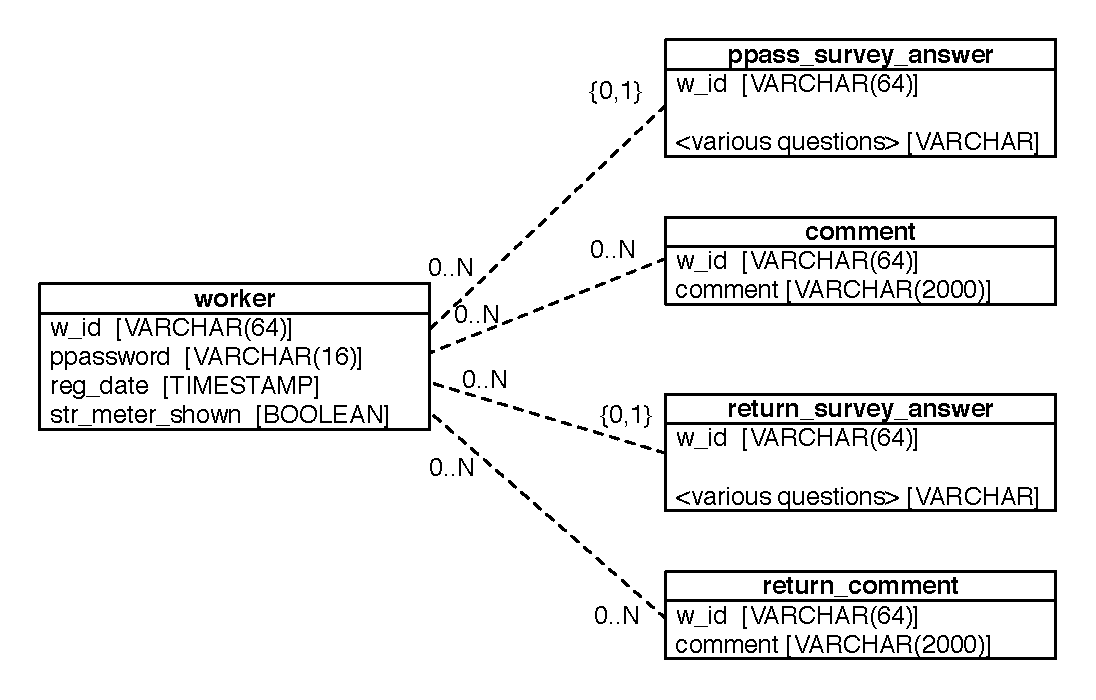
\includegraphics[width=\textwidth]{Images/db_schema}
      \caption{Database Schema}
      \label{fig:db-schema}
    \end{figure}

    \begin{figure}[htpb]
      \centering
      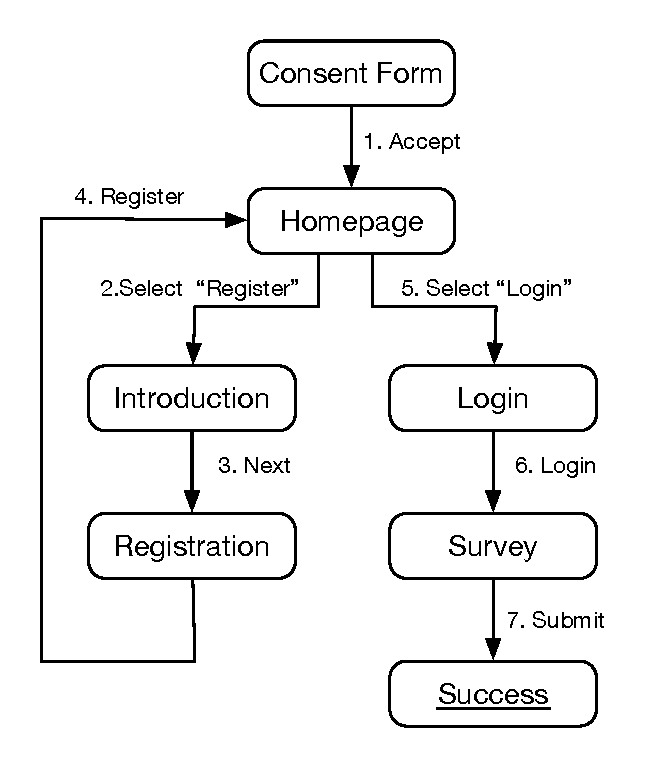
\includegraphics[width=0.55\textwidth]{Images/control_flow}
      \caption{Control flow diagram of website}
      \label{fig:control_flow}
    \end{figure}

    The created website used a simple control flow to emulate a registration process, as seen in Figure~\ref{fig:control_flow}. Images of each webpage can be found in Appendix~\ref{ap:Website}. On the landing page (\ref{aps:consent}), MTurk workers were shown a consent form offering information about the researchers and a security notice, to which they had to agree before they could proceed further. On the \emph{homepage} (\ref{aps:homepage}), they were presented with two buttons, ``Register'' and ``Login''; selecting the former on their first visit would lead them to to \emph{Introduction} page (\ref{aps:intro}). This page explained the task and asked participants to imagine that they were creating a password for their banking account, a notice that prior work has proven to lead to stronger password creation~\cite{pass_policy_new}, and also informed them that they would be asked to return to this website, so they should use their usual methods for remembering and protecting an important password.

    On loading the \emph{Instructions} page, the server would randomly assign them to either the control group (no strength meter) or the experiment group (strength meter shown), and try to asynchronously load the projection dictionary for the latter group, in preparation for the next page. The \emph{Registration} page (\ref{aps:registration}) differed between the conditions, as shown in Figure~\ref{fig:registration} (n.b. the password fields were of type ``text'' instead of ``password'', so users could see their passwords while typing), with the experiment group getting visual feedback on their passwords, as well as the option to get suggestions of strong passwords generated from a dictionary.

    \begin{figure}[H]
      \makebox[\textwidth][c] {
        \begin{subfigure}[t]{0.3\textwidth}
            \includegraphics[width=\textwidth]{Images/1-register-nostr}
            \caption{Without strength meter}
        \end{subfigure}
        ~
        \begin{subfigure}[t]{0.3\textwidth}
            \includegraphics[width=\textwidth]{Images/1-register-meter}
            \caption{With strength meter}
        \end{subfigure}
        ~
        \begin{subfigure}[t]{0.3\textwidth}
            \includegraphics[width=\textwidth]{Images/1-register-meter-sugg}
            \caption{With strength meter and password suggestions}
        \end{subfigure}
      }
      \repeatcaption{fig:registration}{Registration page}
    \end{figure}

    After a successful registration, the workers were redirected to the homepage and selected ``Login'', whereupon they were presented with a partial password challenge in the \emph{Login} page (\ref{aps:login}). Following a successful login, the users were asked to complete a survey about their experience and demographics, presented in detail in section~\ref{ssec:usability_setup}, and finally received a completion code, so they could submit their HIT on MTurk.

    \begin{figure}[htpb]
      \makebox[\textwidth][c] {
        \begin{subfigure}[t]{0.4\textwidth}
            \includegraphics[width=\textwidth]{Images/2-login-init}
            \caption{Initial login screen}
        \end{subfigure}
        ~
        \begin{subfigure}[t]{0.4\textwidth}
            \includegraphics[width=\textwidth]{Images/2-login-ppass}
            \caption{Partial password challenge}
        \end{subfigure}
      }
      \repeatcaption{fig:login}{Login page}
    \end{figure}

    The website that we developed was deployed and hosted on the free tier of the OpenShift Online Platform-as-a-Service (PaaS)~\cite{openshift} offered by RedHat, using PostgreSQL~\cite{postgresql} as the database management system (DBMS).
% !TEX root = ../msc_thesis.tex

\chapter{Results}
\label{cha:results}
To the extent of our knowledge and research, no prior work exists that examines strength meters in a partial password setting. The results of our research are therefore the first ones published for this setting and can serve as a baseline for future research on the subject. At the same time, we can indirectly compare our findings with the ones from research on traditional passwords, and examine if some hypotheses hold true in both settings.

The primary goal of this research was to examine the effect of the partial password meter on the strength of the created partial passwords, and secondly, its effect on their memorability. In order to draw conclusions, we formulated and tested the following null hypotheses in the field:

\begin{itemize}
  \item[] $H_{0a}$: Partial passwords are not stronger when the partial password meter is present during creation.
  \item[] $H_{0b}$: Partial passwords are not more memorable when the partial password meter is present during creation.
\end{itemize}

Following the same methodology as Ur et al., we conducted an online study consisting of two parts. Ideally, the study would be conducted with participants that were using partial passwords in their online routine - possibly limiting the demographic to UK residents. An option to gather the necessary data would be to run the experiment in an on-campus laboratory environment, recruiting students and other researchers to participate in the study. We deemed that doing so would restrict us to a very specific demographic, with a distinct age distribution, education level and experience in research studies and could therefore skew the results. In order to align this research as best as possible with previous work, a crowdsourcing platform that uses a mainly UK demographic and on which custom Human Intelligence Tasks can be specified for execution would be an ideal solution. Unfortunately, after examining the available options, none was found that fit the criteria, while also being cost-efficient. Ultimately, we decided recruiting subjects for our study (also referred to as \emph{workers}) from Amazon's MTurk platform, while providing them with a brief introduction and explanation of partial passwords.

Participants were required to be at least 18 years old and use a web browser with enabled JavaScript capabilities. The details for each task are described in the following sections. While not directly mentioning the purpose of the study to the subjects, we did not employ subterfuge to hide it, unlike what Egelman et al. did in their study~\cite{strength_meter_impact}. By saying that ``We are conducting an academic survey about partial challenges on passwords and we are testing a new partial password system.'', participants were made aware of the general focus of this research. Since we were particularly interested in accurately pinpointing the effect the password meter had in the strength of the created passwords, we decided to use a significance level of $\alpha = 0.01$ for that statistical test, in order to minimise the probability of a type I error. For all other statistical tests in our analysis, the common $\alpha = 0.05$ value was used.

\section{Partial password strength metric correctness}
  \label{sec:correctness}
  Before setting out to test the hypotheses, the correctness of the implemented partial password meter needed to be verified. As mentioned in Section~\ref{sec:str_meter_existing}, the term ``password strength'' is ill-defined, which renders a theoretical proof of correctness impossible. In accordance with the definition of password strength we adopted, a practical approach was followed when testing the correctness of the developed meter.

  A Python script containing the partial password strength calculation algorithm described in Section~\ref{ssec:str_metric} combined with a projection dictionary generated by the RockYou dataset was used to evaluate the password strength of different password lists. The password lists tested were the password database leaks from the RockYou website and the PHPBB forums, as well as the top 10 million passwords dictionary released in 2015~\cite{top10m_pass}, a revision of the top-500~\cite{top500_pass} and top-10000~\cite{top10000_pass} password lists released in 2005 and 2011, respectively. For each set, we filtered out the passwords that did not meet the specified length (6-15 characters) and discovered the most common password that was ranked as ``Strong'' or ``Very Strong'' from our algorithm. The Python CLI version of the strength meter was used for faster and more flexible offline evaluation of the aforementioned dictionaries - the algorithm and scores are consistent between the Python and JS implementations.

  The findings of the aforementioned analysis are displayed in Table~\ref{tab:str_correct}. We observe that the algorithm is adequately strict in the ranking of partial passwords, even when testing other datasets. It is worth noting, that while these passwords seem and are weak in a traditional setting with offline dictionary attacks, the chance of successfully guessing a partial password challenge of them within $\beta = 10$ max guesses in an online attack scenario is minuscule. We conclude therefore that the strength metric's performance is acceptable and can be used to test the selected hypotheses.

  \begin{table}[htpb]
    \centering
    \small
    \hspace*{-1.5cm}
    \begin{tabular}{|c||c|c|c|c|c|c|}
      \hline
      \textbf{Dataset} & \multicolumn{2}{|c|}{\textbf{RockYou}} & \multicolumn{2}{|c|}{\textbf{PHPBB}} & \multicolumn{2}{|c|}{\textbf{top 10M}} \\
      \hline
      \textbf{Verdict} & \textbf{Strong} & \textbf{Very Strong} & \textbf{Strong} & \textbf{Very Strong} & \textbf{Strong} & \textbf{Very Strong} \\
      \hline
      \textbf{\# of passwords} & \multicolumn{2}{|c|}{31063584} & \multicolumn{2}{|c|}{230905} & \multicolumn{2}{|c|}{9061038} \\ \hline
      \textbf{Most common} & \multicolumn{2}{|c|}{50cent} & \multicolumn{2}{|c|}{qazwsx} & 696969 & 1qaz2wsx \\ \hline
      \textbf{Frequency} & \multicolumn{2}{|c|}{3294} & \multicolumn{2}{|c|}{92} & 3050 & 2531 \\ \hline
      \textbf{\% frequency} & \multicolumn{2}{|c|}{0.011\%} & \multicolumn{2}{|c|}{0.040\%} & 0.034\% & 0.028\% \\ \hline
    \end{tabular}
    \caption{Most common password ranked ``Strong'' or ``Very Strong'' per dataset}
    \label{tab:str_correct}
  \end{table}

\section{Effect on partial password strength}
  \label{sec:useability}

  \subsection{Methodology}
    \label{ssec:useability_setup}
    We recruited 200 participants from Amazon MTurk to participate in this research. For the first part of the study, subjects were paid 75 cents and were asked to ``Answer a survey about partial passwords after completing a mock registration process''. In order to qualify for the task, they had to complete a small screener test that ensured they were able to correctly answer partial password challenges. This qualification test also served to prime workers for the task and inform them about the concept of partial passwords, since most of them were expected to not have experience with partial password login systems, as our prior survey indicated (described in Section~\ref{sssec:partial_pass_extent_use}). Before the task was published, a small-scale (20 subjects, both MTurk workers and university students) pilot was carried out, in order to discover possible bugs or other problems with the website. Since the feedback received from this pilot run motivated changes in the website and the strength meter, we discarded their results to ensure consistency within the study samples. The participants in our study were heavily based in the US (183/200, 91.5\%), and had a 60/40 Men/Women ratio. Ages varied from 18-69, having a mean age of 32.77 with 10.07 standard deviation and with 46.5\% of the participants being in the 26-35 age range.

    Participants were randomly assigned to either the control or the experiment condition and were asked to complete a registration process on our website, followed by a successful login using a partial challenge on their passwords, as shown in the control flow in Figure~\ref{fig:control_flow}. After successfully logging in, they were presented with a survey containing questions about their opinions concerning the strength meter (this group of questions differed between conditions), questions about the partial password and their method of answering the challenge, as well as some basic demographic questions. The multiple-choice survey questions were presented in a equidistant (neutral) manner and designed to offer five-level Likert-type scale responses~\cite{likert}, in order to minimise user bias. An \emph{attention-check} question (a question with a clear, predefined answer) was also inserted in the survey, to reduce the likelihood of a worker randomly or automatically (with a script) completing the questionnaire. The full survey is included in Appendix~\ref{aps:survey_useability}.
    % Finally, the question order and wording was selected as to introduce cross-coding, meaning that an average subject would not select the same column (value) or even side for answering all questions.

  \subsection{Results}
    \label{ssec:useability_results}
    Due to the way partial password strength is calculated, scores > 100 are possible, so during the processing of the results we normalised all password strength scores over that threshold to 100. We categorised the created partial passwords depending on their strength rating, using the same thresholds specified for the strength meter, and counted the occurrences for each on both conditions. This process was used to get a better overview and visualisation of the meter's effect, the results are presented in Table~\ref{tab:verdict} and Figure~\ref{fig:verdict}.

    \begin{table}[htpb]
      \hspace*{-1.5cm}
      \begin{minipage}[b]{0.3\linewidth}
        \centering
        \scriptsize
        \begin{tabular}{ l r r}
          \toprule
          \textbf{Verdict} & \textbf{Meter} & \textbf{No Meter} \\ \midrule
          \textbf{Very Strong} & 70 & 57 \\
          \textbf{Strong} & 8 & 5 \\
          \textbf{Good} & 11 & 10 \\
          \textbf{Fair} & 7 & 16 \\
          \textbf{Weak} & 4 & 12 \\ \midrule
          \textbf{Total} & 100 & 100 \\ \bottomrule
        \end{tabular}
          \caption{Verdict frequencies}
          \label{tab:verdict}
      \end{minipage}\hfill
      \begin{minipage}[b]{0.7\linewidth}
        \centering
        \includegraphics[width=\linewidth]{Images/results-str}
        \captionof{figure}{Pie charts of verdict frequencies}
        \label{fig:verdict}
      \end{minipage}
    \end{table}

    From the generated overview, a noticeable effect on the partial password strength can be observed. In order to test the null hypothesis $H_{0a}$, we performed a t-test on the normalised partial password strengths. The samples from the two groups of participants are considered independent and identically distributed, so we use the unpaired, two-sample, unequal variance test (Welch's t-test) with two tails. As we previously mentioned, for this test we had decided (\emph{a priori}) to use a significance level of $\alpha = 0.01$.

    Judging from the results of this process, which is presented in Table~\ref{tab:t-test}, we observe that the t-statistic of the experimental data is over the critical value. We therefore \textbf{reject the null hypothesis $H_{0a}$ (with 99\% confidence) and claim that the partial password strength meter has a measurable positive effect in the strength of the created partial passwords}.

    \begin{table}[htpb]
      \centering
      \begin{tabular}{l r r}
      \toprule
      & \textbf{Meter} & \textbf{No Meter} \\
      \midrule
      \textbf{Mean $(\overline{X})$} & 86.2767 & 75.3703 \\
      \textbf{Variance ($\sigma^2$)} & 577.7259 & 1061.4647 \\
      \textbf{\# of Observations} & 100 & 100 \\
      \midrule
      \textbf{Hypothesised mean difference} & \multicolumn{2}{c}{0} \\
      \textbf{Degrees of freedom ($df$)} & \multicolumn{2}{c}{182} \\
      \textbf{t-statistic} & \multicolumn{2}{c}{2.6938} \\
      \textbf{$P(T\leq t)$ two-tail} & \multicolumn{2}{c}{0.0077} \\
      \textbf{t critical two-tail} & \multicolumn{2}{c}{2.6031} \\
      \bottomrule
      \end{tabular}
      \caption{t-Test: Two-Sample - Unequal Variances, $\alpha = 0.01$}
      \label{tab:t-test}
    \end{table}

    Apart from the main hypothesis that was tested, the answers in the study offer insight in various other aspects of partial passwords. Testing for differences between demographics indicated that there was no significant variation in strength between men and women and neither age seemed to affect partial password strength. Participants aged 55+ had a 12\% higher than average score, but the population sample is small enough (8) that it can likely be statistical noise. Similarly, workers from India had a lower than average password strength (69.34), but the small sample (9) does not allow us to draw any conclusions.

    The experiment and control group displayed a similar distribution in their perceptions of their own password's resilience against partial attacks, both being in general more pessimistic than what the meter suggested (or would have suggested, in the case of the control group). This similar distribution in perceived strength, combined with the significant differences in the actual password strength leads to the control group displaying a slightly positive correlation (+0.225 factor) between perceived and actual strength, while the experiment group having practically no correlation at all (-0.076 factor). This comes as a surprise, considering that 60\% of the experiment group indicated that they did not believe the strength meter gave an incorrect score to their password, and only 19\% disagreed with the displayed score.\footnote{When values do not sum to 100\%, the difference exists in the \emph{Neutral} response of the scale.}

    A question in the survey concerned the methods subjects used to count the characters, when answering the partial password challenge; this is of particular interest, since it a unique feature that applies only to partial passwords. We discovered that the subjects' methods of counting the characters did not differ significantly between conditions, as shown in Figure~\ref{fig:counting-methods}. Mental counting appears as the main method of counting with 42\% of the total subjects reporting to use it, counting with fingers came second with 32\%, while counting while seeing the password came at a close third, with 26\% of participants.

    \begin{figure}[htpb]
      \centering
      \includegraphics[width=\textwidth]{Images/counting}
      \caption{Counting methods for the partial password challenge}
      \label{fig:counting-methods}
    \end{figure}

    As this project lies at the intersection of computer security with HCI, it is important to examine the strength meter from a useability perspective, and the first questions in this survey were designed to help do so. Participants in the experiment group were asked to indicate their level of agreement on statements concerning the helpfulness of the password meter on creating stronger passwords, the importance of getting a high rating, the annoyance caused by it and their judgement of its correctness. Subjects in the control group were asked similar questions, but for strength meters in general; the exact wording of the statements can be found in Appendix~\ref{aps:survey_useability}, and the results are presented in Table~\ref{tab:beliefs}.

    \begin{table}[htpb]
      \centering
      \scriptsize
      \hspace*{-2cm}
      \begin{tabular}{p{3cm} rrrrrrrr}
        \toprule
         & \multicolumn{2}{c}{\textbf{Helpfulness}} & \multicolumn{2}{c}{\textbf{Importance}} & \multicolumn{2}{c}{\textbf{Annoyance}} & \multicolumn{2}{c}{\textbf{Incorrect results}} \\
        \textbf{Level of Agreement} & \textbf{Meter} & \textbf{No meter} & \textbf{Meter} & \textbf{No meter} & \textbf{Meter} & \textbf{No meter} & \textbf{Meter} & \textbf{No meter} \\
        \midrule
         \textbf{Strongly Agree} & 17 & 13 & 25 & 19 & 2 & 15 & 6 & 5 \\
         \textbf{Agree} & 46 & 52 & 44 & 31 & 5 & 20 & 13 & 22 \\
         \textbf{Neither Agree \newline or Disagree} & 20 & 14 & 16 & 24 & 11 & 7 & 21 & 27 \\
         \textbf{Disagree} & 13 & 18 & 9 & 21 & 40 & 41 & 42 & 40 \\
         \textbf{Strongly Disagree} & 4 & 3 & 6 & 5 & 42 & 17 & 18 & 6\\
        \bottomrule
      \end{tabular}
      \caption{Participants' beliefs about password meter}
      \label{tab:beliefs}
    \end{table}

    We can observe that the subjects in the \emph{Meter} condition had a generally positive experience with the partial password strength meter. 63\% of them reported that it helped them select a stronger password, with only 17\% claiming it did not help them, while the vast majority 80\% did not consider it annoying. Running omnibus ($\chi^2$ goodness of fit) tests between the groups, we discovered that a borderline significant difference ($p=0.048$) difference exists on how important a high score on the displayed strength meters is. Accounting for the bias introduced by the fact that object of the research was clear to the participants, we suggest not accepting this result as significant, as to avoid type I errors. A certain difference between the groups was observed in the annoyance caused by this vs password meters in general, with a probability $p=0.0000040 \ll \alpha = 0.05$. The margin is large enough for us to safely conclude that there is a significant difference in that aspect, but we need to keep in mind that possible confusions between \emph{``password meter''} and \emph{``password policy''} might have influenced the results of the control group.

\section{Effect on partial password memorability}
  \label{sec:memorability}
  In this section, we detail the methodology followed while testing the $H_{0b}$ null hypothesis, and report our results, as well as other findings that emerged from the analysis of the collected data.

  \subsection{Methodology}
    \label{ssec:memorability_setup}
    Four days after each participant's completion of the task, they were sent an email informing them about a new, follow-up survey that they could return and complete. For the final part of the study, workers were compensated with 10 cents for attempting to login, while those who were able to remember their password and successfully login were granted a bonus of 22 cents, as advertised. This reward allocation method was used in order to give MTurk workers a monetary incentive to try and recall their passwords, as Ipeirotis discovered that one of their primary motivations is the financial compensation~\cite{mturk_demographic}. At the same time this allocation was fair, since workers who forgot their passwords were not presented with a survey and consequently spent less time on the HIT.

    Participants were asked to return to our website and answer a short survey, which was presented to them after a successful login using a partial password challenge. It was made clear to them (in the HIT instructions) that they would be able to complete the task regardless of their ability to recall their passwords, by clicking on a ``Forgot Password'' link, forfeiting the bonus. This was done in order to reassure them and encourage the participation of the subjects that had since forgotten their passwords \footnote{N.B. the HIT approval rate \% is an important metric in the MTurk platform, so workers generally avoid HITs they fear failing}. It is imperative to note here that during the first part of the study subjects \textbf{were informed} that they would need to remember their passwords for future use and asked to employ their usual methods for remembering and protecting an important password.

    From the 200 participants invited, 144 returned to complete the second part of the study. Those that succeeded in recalling their password were asked questions about the difficulty in recalling it, the method they used to remember it and (again) the method of counting the characters for the partial challenge. They were also asked how many unsuccessful attempts they made before logging in; this is something that can be measured server-side but it was not implemented and the work by Ur et al. indicated that workers were generally honest when answering those questions, with only 1.6\% found lying in their responses~\cite{strength_meter_effect}.

  \subsection{Results}
    \label{ssec:memorability_results}

    The analysis began similarly with the first stage, by counting and grouping the results in order to get an overview of the meter's effect; the values are presented in Table~\ref{tab:memorability}. We observe that participants from both conditions were equally likely to accept the return HIT, which is in agreement with our expectations and that there is a very slight increase in memorability for subjects in the \emph{Meter} condition.

    \begin{table}[htpb]
      \centering
      \begin{tabular}{l rrr}
      \toprule
      & \textbf{Meter} & \textbf{No meter} & \textbf{Total} \\
      \midrule
       \textbf{Remembered} & 52 & 47 & 99 \\
       \textbf{Forgot} & 24 & 21 & 45 \\
       \textbf{Returned} & 73 & 71 & 144 \\
       \textbf{Remembered \%} & 71.23 & 66.20 & 68.75 \\
      \bottomrule
      \end{tabular}
      \caption{Memorability of partial passwords}
      \label{tab:memorability}
    \end{table}

    In order to examine the null hypothesis $H_{0b}$, we performed an omnibus ($\chi^2$ goodness of fit) test on the actual and expected values. The calculated probability was $p=0.51$, indicating that there is a high probability that the differences were simply statistical noise; we therefore claim that we did not observe a significant effect of the partial password strength meter on the memorability of partial passwords and \textbf{accept $H_{0b}$}.

    After examining the collected data, there are other interesting observations to be made. As shown in Table~\ref{tab:remember}\footnote{Sum of values is larger than the number of subjects that remembered their passwords, as they were asked to ``select all that apply''} (and the accompanying Figure~\ref{fig:remember}), the main method of remembering was memorising the password (67\%), with writing them down being the second most frequent way (21\%). Ur et al.'s findings were that 38.0\% of the participants that returned had stored their passwords, either electronically or on paper, a value that does not significantly differ from our data (32.7\%), reinforcing our belief in the validity of the collected data. The results of $\chi^2$ tests on our data determined that the proportion of participants using each method did not differ between conditions ($p=0.741$), an outcome that also is in agreement with their findings. Two users who selected the ``Other'' option reported sending an email containing the password to themselves and taking a photo of the password using their mobile phones. It is regrettable to notice that only a very small portion of subjects in our sample employ password management software (e.g. KeePass, LastPass, 1Password etc), which was one of the most common suggestions security experts offered with regard to best online security practices~\cite{security_practices_experts}.

    \begin{table}[htpb]
      \begin{minipage}[b]{0.42\linewidth}
        \centering
        \small
        \begin{tabular}{l r}
          \toprule
          \textbf{Method} & \textbf{Count} \\ \midrule
          \textbf{Memorised} & 74 \\
          \textbf{Wrote down} & 23 \\
          \textbf{Stored in file} & 5 \\
          \textbf{Password manager} & 5 \\
          \textbf{Other} & 3 \\ \bottomrule
        \end{tabular}
          \caption{Remembering methods}
          \label{tab:remember}
      \end{minipage}\hfill
      \begin{minipage}[b]{0.55\linewidth}
        \centering
        \includegraphics[width=\linewidth]{Images/remember-method}
        \captionof{figure}{Pie chart of remembering methods}
        \label{fig:remember}
      \end{minipage}
    \end{table}

    Because of the partial password setting of the study, we chose to examine changes in the ways participants used to count the characters between the first and second stage. As seen in Table~\ref{tab:counting_changes}, subjects who counted the characters in their minds or while seeing them did not significantly change their behaviour; 78.1\% and 80.6\% of them, respectively, reported using the same method between the two stages of the study. On the other hand, only 64.7\% of the subjects that counted using their fingers indicated that they used the same method the second time they logged in. From the workers that changed their way of counting, we observed that most switched to counting while seeing the password, with the ``changed'' users constituting the 34.2\% of the total number or subjects found using the method; the corresponding percentages were 21.9\% and 18.5\% for mental and finger counting. This behaviour can possibly be attributed to the subjects storing or writing the passwords down as a means to remember it - the coinciding numbers of those that somehow stored their password (36) with those that reported counting while seeing the password (38) further strengthen this assumption.


    \begin{table}[htpb]
      \centering
      \small
      \begin{tabular}{l rrr}
      \toprule
      \textbf{From/To} & \textbf{Mental} & \textbf{Fingers} & \textbf{Seeing pass} \\
      \midrule
       \textbf{Mental} & 25 & 2 & 5 \\
       \textbf{Fingers} & 4 & 22 & 8 \\
       \textbf{Seeing pass} & 3 & 3 & 25 \\
      \bottomrule
      \end{tabular}
      \caption{Changes in counting methods for partial password challenges}
      \label{tab:counting_changes}
    \end{table}

    % TODO: reset count-forgot correlation?

% !TEX root = ../msc_thesis.tex

\chapter{Conclusion}
\label{cha:conclusion}

  \section{Project Evaluation}
    \label{sec:evaluation}

  \section{Limitations}
    \label{sec:limitations}
    self-selection bias from HIT description, MTurk workers not familiar with ppass, run on UK demographic, meter effect during pass creation (not only final result), also measure time spent selecting password, edit distance etc. Dictionary needs to be constantly updated.

  \section{Ethical considerations}
    \label{sec:ethical}
    Everyone has rockyou,phpbb, top 10M so no problem! we did not use the linkedin as it was recent and we did not want to attract further attention to it.

  \section{Future work}
    \label{sec:future_work}

    \subsection{Possible improvements on strength meter}
      \label{ssec:meter_improvements}
      Experimental studies to find a better set of rules.

    \subsection{Partial password attack improvements}
      \label{ssec:attack_improvements}
      Continue work on the paper by D. Aspinall and M. Just~\cite{part_pass}.

      Take into account password policies when generating dictionary.

      \begin{itemize}
        \item Case where N=62, n>X. (maximum letter position asked is useful metadata!)
        \item Using letters outside of challenge to make better guesses (e.g. knowing \#1=`1', \#2=`2' and \#5=`5', I can make a good guess for 3,4,6 even at w0.)
      \end{itemize}

    \subsection{Secure partial passwords storage}
      \label{ssec:secure_store}
      Common passwords: salted hash (bcrypt). Because of their unique characteristic in the form partial challenges, they are in cleartext - or posibly encrypting all 3-letter challenges - trivially brute forceable. This is VERY bad in case of db leak.

      Reversible encryption as a solution?

%% Appendices
\begin{appendices}
% !TEX root = ../msc_thesis.tex

\chapter{Partial password strength meter surveys}
  \label{ap:Surveys}
  \section{Survey about the extent of use of partial password challenges}
    \label{aps:survey_extent}
    \includepdf{Images/survey-ppass-world-use.png}

  \section{Survey about the useability of the partial password strength meter}
    \label{aps:survey_useability}

    \subsection{MTurk HIT}
      \label{apss:useability_hit}

      \subsubsection{Description}
        \label{apsss:useability_hit_descr}
        Answer a survey about partial passwords after completing a mock registration process [~5 minutes] (the registration is used exclusively for this research and only asks for Worker ID - no identifiable information is required).

      \subsubsection{Instructions}
        \label{apsss:useability_hit_instr}
        We are conducting an academic survey about partial challenges on passwords and we are testing a new partial password system.

        \textbf{``\emph{Partial Password Challenges}'' refers to challenges of the form ``Please enter characters in positions 3, 4 and 6 of your password/PIN''.}

        You will \textbf{NOT} be asked to provide any identifiable information or credentials.

        Please visit the link below (note that \underline{JavaScript needs to be enabled}), register with the website and then login to complete a short survey. At the end of the survey, you will receive a code to paste into the box below to receive credit for taking our survey.

        \textbf{Make sure to leave this window open as you complete the survey}. When you are finished, return to this page to paste the code into the box.

        Note that only one submission per worker will be accepted.


    \subsection{Questions}
    \label{apss:useability_questions}
    {\setmainfont[Mapping=TeX-text,Ligatures=TeX]{Helvetica}
    \textbf{Q1. To what extent do you agree or disagree with each of the following statements?}
      \begin{table}[H]
        \centering
        \scriptsize
        \hspace*{-1cm}
        \begin{tabular}{|P{6.8cm}|P{1.6cm}|P{1.1cm}|P{2.2cm}|P{0.8cm}|P{1.3cm}|}
        \hline
         & \textbf{Strongly Disagree} & \textbf{Disagree} & \textbf{Neither Agree or Disagree} & \textbf{Agree} & \textbf{Strongly Agree} \\
        \hline
        \textbf{The password strength meter helped me select a stronger password.} & $\ocircle$ & $\ocircle$ & $\ocircle$ & $\ocircle$ & $\ocircle$ \\
        \hline
          \textbf{I think the password strength meter gave an incorrect score of my password's strength.} & $\ocircle$ & $\ocircle$ & $\ocircle$ & $\ocircle$ & $\ocircle$ \\
        \hline
          \textbf{It is important to me that the password strength meter gives my password a high score.} & $\ocircle$ & $\ocircle$ & $\ocircle$ & $\ocircle$ & $\ocircle$ \\
        \hline
          \textbf{Please select ``Agree''.} & $\ocircle$ & $\ocircle$ & $\ocircle$ & $\ocircle$ & $\ocircle$ \\
        \hline
        \textbf{The password strength meter was annoying.} & $\ocircle$ & $\ocircle$ & $\ocircle$ & $\ocircle$ & $\ocircle$ \\
        \hline
        \end{tabular}
        \caption{Experiment group (with strength meter)}
      \end{table}

      \begin{table}[H]
        \centering
        \scriptsize
        \hspace*{-1cm}
        \begin{tabular}{|P{6.8cm}|P{1.6cm}|P{1.1cm}|P{2.2cm}|P{0.8cm}|P{1.3cm}|}
        \hline
         & \textbf{Strongly Disagree} & \textbf{Disagree} & \textbf{Neither Agree or Disagree} & \textbf{Agree} & \textbf{Strongly Agree} \\
        \hline
        \textbf{A password strength meter would have helped me select a stronger password.} & $\ocircle$ & $\ocircle$ & $\ocircle$ & $\ocircle$ & $\ocircle$ \\
        \hline
          \textbf{I think that password strength meters generally give an incorrect score of my password's strength.} & $\ocircle$ & $\ocircle$ & $\ocircle$ & $\ocircle$ & $\ocircle$ \\
        \hline
          \textbf{It is important to me that password strength meters give my password a high score.} & $\ocircle$ & $\ocircle$ & $\ocircle$ & $\ocircle$ & $\ocircle$ \\
        \hline
          \textbf{Please select ``Agree''.} & $\ocircle$ & $\ocircle$ & $\ocircle$ & $\ocircle$ & $\ocircle$ \\
        \hline
        \textbf{I generally consider password strength meters to be annoying.} & $\ocircle$ & $\ocircle$ & $\ocircle$ & $\ocircle$ & $\ocircle$ \\
        \hline
        \end{tabular}
        \caption{Control group (without strength meter)}
      \end{table}

    \textbf{Q2. How difficult do you believe it would be for a malicious person to correctly guess the three requested letters from your password?}
    \begin{shortitemize}
      \item[$\ocircle$] Very Difficult
      \item[$\ocircle$] Dificult
      \item[$\ocircle$] Neutral
      \item[$\ocircle$] Easy
      \item[$\ocircle$] Very Easy
    \end{shortitemize}

    \textbf{Q3. Do you use the partial password you selected for any accounts on other websites?}
    \begin{shortitemize}
      \item[$\ocircle$] Yes
      \item[$\ocircle$] No
    \end{shortitemize}

    \textbf{Q4. How did you count the characters to answer the partial password challenge?}
    \begin{shortitemize}
      \item[$\ocircle$] I counted in my mind.
      \item[$\ocircle$] I counted using my fingers.
      \item[$\ocircle$] I counted while seeing the password (e.g. on screen or written on paper).
      \item[$\ocircle$] Other (please specify): \ovalbox{\phantom{A box for some explanation goes here}}
    \end{shortitemize}

    \textbf{Q5. Thinking back over the past year of using your partial passwords, how many times did you need to reset them (use the ``forgot password'' feature)?}
    \begin{shortitemize}
      \item[$\ocircle$] N/A
      \item[$\ocircle$] 0
      \item[$\ocircle$] 1
      \item[$\ocircle$] 2
      \item[$\ocircle$] 3
      \item[$\ocircle$] More than 3
    \end{shortitemize}

    \textbf{Q6. What is your age?} \ovalbox{\phantom{box here}}

    \textbf{Q7. What is your gender?}
    \begin{shortitemize}
      \item[$\ocircle$] Male
      \item[$\ocircle$] Female
      \item[$\ocircle$] Prefer not to answer
    \end{shortitemize}

    \textbf{Q8. What is your nationality?} \ovalbox{\phantom{A box goes here}}

    \textbf{Q9. What is your country of residence?} \ovalbox{\phantom{A box goes here}}

    \textbf{Q10. How often do you login to online banking services that require a reply to a partial password challenge?}
    \begin{shortitemize}
      \item[$\ocircle$] Daily
      \item[$\ocircle$] Weekly
      \item[$\ocircle$] Monthly
      \item[$\ocircle$] Less frequently
      \item[$\ocircle$] Never
    \end{shortitemize}
    }

  \section{Return survey about the memorability of partial passwords}
    \label{aps:survey_memorability}

      \textbf{Invitation email}
      \begin{quote}
      Greetings,

      You are invited to take part in another survey regarding partial passwords. You have been awarded the required qualification and you should be able to view and accept the HIT in the following link, provided your HIT approval rate remains above 97\%\\
      \href{https://www.mturk.com/mturk/searchbar?requesterId=A6N1BQ2VBW7RS}{https://www.mturk.com/mturk/searchbar?requesterId=A6N1BQ2VBW7RS}

      You can complete the HIT even if you cannot remember your password, but there is a significant bonus for those who can, so we suggest you try to recall it.

      Thank you for your contributions in our research.
      \end{quote}

    \subsection{MTurk HIT}
      \label{apsss:memorability_hit}

    \subsubsection{Description}
      \label{apsss:memorability_hit_descr}
      Return to the website where you created a password a few days ago and answer a small survey about remembering passwords. \$0.22 bonus for workers that remember their password. [1-2 minutes]

    \subsubsection{Instructions}
      \label{apsss:memorability_hit_instr}
      We are conducting an academic survey about the memorability of passwords used for partial password challenges.

      \textbf{``\emph{Partial Password Challenges}'' refers to challenges of the form ``Please enter characters in positions 3, 4 and 6 of your password''.}

      Please visit the link below (note that \underline{JavaScript needs to be enabled}), login using the password you created a few days ago, and complete a short survey (5 questions). At the end, you will receive a code to paste into the box below to receive credit for taking our survey.

      If you cannot remember your password, click at the ``\emph{Forgot password?}'' link at the login page (after you enter your Worker ID) to get the survey code, \underline{\textbf{forfeiting the \$0.22 bonus}}.

      \textbf{Make sure to leave this window open as you complete the survey.} When you are finished, return to this page to paste the code into the box.

      Note that only one submission per worker will be accepted.

    \subsection{Questions}
    \label{apss:memorability_questions}
    {\setmainfont[Mapping=TeX-text,Ligatures=TeX]{Helvetica}
    \textbf{Q1. How difficult was it to recall the password?}
    \begin{shortitemize}
      \item[$\ocircle$] Very Difficult
      \item[$\ocircle$] Dificult
      \item[$\ocircle$] Neutral
      \item[$\ocircle$] Easy
      \item[$\ocircle$] Very Easy
    \end{shortitemize}

    \textbf{Q2. How did you remember your password (select all that apply)?}
    \begin{shortitemize}
      \item[$\Box$] I memorized it.
      \item[$\Box$] I wrote it down.
      \item[$\Box$] I stored it in a file (on my computer / USB stick / other).
      \item[$\Box$] I saved it in a Password Manager (e.g. browser's password manager, LastPass, KeePass, 1Password, etc.).
      \item[$\Box$] Other (please specify): \ovalbox{\phantom{A box for some explanation goes here}}
    \end{shortitemize}

    \textbf{Q3. How did you count the characters to answer the partial password challenge?}
    \begin{shortitemize}
      \item[$\ocircle$] I counted in my mind.
      \item[$\ocircle$] I counted using my fingers.
      \item[$\ocircle$] I counted while seeing the password (e.g. on screen or written on paper).
      \item[$\ocircle$] Other (please specify): \ovalbox{\phantom{A box for some explanation goes here}}
    \end{shortitemize}

    \textbf{Q4. How many (failed) login attempts did you make, before successfully logging in?}
    \begin{shortitemize}
      \item[$\ocircle$] 0
      \item[$\ocircle$] 1
      \item[$\ocircle$] 2
      \item[$\ocircle$] 3
      \item[$\ocircle$] More than 3
    \end{shortitemize}

    \textbf{Q5. Do you use this password for any accounts on other websites?}
    \begin{shortitemize}
      \item[$\ocircle$] Yes
      \item[$\ocircle$] No
    \end{shortitemize}
    }
% !TEX root = ../msc_thesis.tex

\chapter{Project Website}
  \label{ap:Website}

  \section{Consent Form}
    \label{aps:consent}
    You are being invited to participate in this academic study. This study is being done by Vasilis Gerakaris as part of a MSc Project under the supervision of professor \href{http://homepages.inf.ed.ac.uk/da/}{David Aspinall} for the \href{http://www.ed.ac.uk/}{University of Edinburgh}.

    If you agree to take part in this study, you will be asked to complete an online survey/questionnaire after completing a mock registration process.

    The selected partial password (memorable information) will stored in cleartext (not encrypted) in our database. In simple terms, this means that we will be able to see the password you have selected.

    While we do not retain any identifying information other than your Worker ID, we strongly suggest that you do \textbf{not} select a password you already use on other accounts.

    We believe there are no known risks associated with this research study; however, as with any online related activity the risk of a breach of confidentiality is always possible. To the best of our ability your answers in this study will remain confidential. After the experiment has concluded and statistical results have been generated, all stored information will be permanently deleted.

    If you have questions about this project or if you have a research-related problem, you may contact the researcher, Vasilis Gerakaris at the following email address: \texttt{s1568962@sms.ed.ac.uk}

    By clicking ``Accept'' below you are indicating that you are at least 18 years old, have read and understood this security notice and agree to participate in this research study. Feel free to print a copy of this page for your records.

  \section{Home page}
    \label{aps:homepage}
    \begin{figure}[H]
      \makebox[\textwidth][c] {
        \includegraphics[width=1.3\textwidth]{Images/0-home}
      }
      \caption{Homepage}
      \label{fig:home}
    \end{figure}

  \section{Introduction}
    \label{aps:intro}
    Imagine that the following is part of the registration process for a bank. The memorable information you select will be used to access online banking services. You will be asked to use this memorable information in a few days to log in again, so it is important that you remember it. Please take the steps you would normally take to remember and protect this information as you would normally protect the ones for your bank account. Behave as you would if this were your real banking credentials.\\

    Do not select a password you already use on other accounts, as I will be able to see them (they are stored in cleartext, not encrypted).

  \section{Registration page}
    \label{aps:registration}
    \begin{figure}[H]
      \makebox[\textwidth][c] {
        \begin{subfigure}[t]{0.4\textwidth}
            \includegraphics[width=\textwidth]{Images/1-register-nostr}
            \caption{Without strength meter}
            \label{fig:reg-nostr}
        \end{subfigure}
        ~ %add desired spacing between images, e. g. ~, \quad, \qquad, \hfill etc.
        \begin{subfigure}[t]{0.4\textwidth}
            \includegraphics[width=\textwidth]{Images/1-register-meter}
            \caption{With strength meter}
            \label{fig:reg-str}
        \end{subfigure}
        ~
        \begin{subfigure}[t]{0.4\textwidth}
            \includegraphics[width=\textwidth]{Images/1-register-meter-sugg}
            \caption{With strength meter and password suggestions}
            \label{fig:reg-str-sugg}
        \end{subfigure}
      }
      \caption{Registration page}\label{fig:registration}
    \end{figure}

  \section{Login page}
    \label{aps:login}
    \begin{figure}[H]
      \makebox[\textwidth][c] {
        \begin{subfigure}[t]{0.4\textwidth}
            \includegraphics[width=\textwidth]{Images/2-login-init}
            \caption{Initial login screen}
            \label{fig:login-init}
        \end{subfigure}
        ~
        \begin{subfigure}[t]{0.4\textwidth}
            \includegraphics[width=\textwidth]{Images/2-login-ppass}
            \caption{Partial password challenge}
            \label{fig:login-ppass}
        \end{subfigure}
        ~
        \begin{subfigure}[t]{0.4\textwidth}
            \includegraphics[width=\textwidth]{Images/2-login-ppass-forgot}
            \caption{Partial password challenge with ``Forgot password'' option}
            \label{fig:login-forgot}
        \end{subfigure}
      }
      \caption{Login page}\label{fig:login}
    \end{figure}

  \section{Completion page}
    \label{aps:complete}
    \begin{figure}[H]
      \centering
      \includegraphics[width=\textwidth]{Images/3-success}
      \caption{Completion page}
      \label{fig:complete}
    \end{figure}
\end{appendices}

%% Choose your favourite bibliography style here.
% \nocite{*}  % Include uncited bibliography
\bibliographystyle{ieeetr}

%% If you want the bibliography single-spaced (which is allowed), uncomment the next line.
% \singlespace

%% Specify the bibliography file. Default is thesis.bib
\bibliography{msc_thesis}

\end{document}
